\section{\label{sec:level1}Observation and Analysis}
\subsection{Magnetoresistance}
\subsubsection{I=198.5mV}
table 1.
\begin{table}[!ht]
    \centering
    \begin{tabular}{|l|l|l|l|}
    \hline
        H(gauss) & Voltage(mv) & Resistance & deltaR/R \\ \hline
        0 & 0.036 & 0.000183861 & 0 \\ \hline
        390 & 0.037 & 0.000188968 & 0.026291892 \\ \hline
        2410 & 0.038 & 0.000194076 & 0.051915789 \\ \hline
        3480 & 0.041 & 0.000209397 & 0.121287805 \\ \hline
        4090 & 0.043 & 0.000219612 & 0.16215814 \\ \hline
        4380 & 0.044 & 0.000224719 & 0.1812 \\ \hline
        4520 & 0.046 & 0.000234934 & 0.2168 \\ \hline
        4560 & 0.048 & 0.000245148 & 0.249433333 \\ \hline
        4700 & 0.049 & 0.000250255 & 0.26475102 \\ \hline
        4920 & 0.05 & 0.000255363 & 0.279456 \\ \hline
        5060 & 0.051 & 0.00026047 & 0.293584314 \\ \hline
        5130 & 0.052 & 0.000265577 & 0.307169231 \\ \hline
        5290 & 0.053 & 0.000270684 & 0.320241509 \\ \hline
        5360 & 0.054 & 0.000275792 & 0.33282963 \\ \hline
    \end{tabular}
\end{table}

\begin{figure}[h!]
\centering
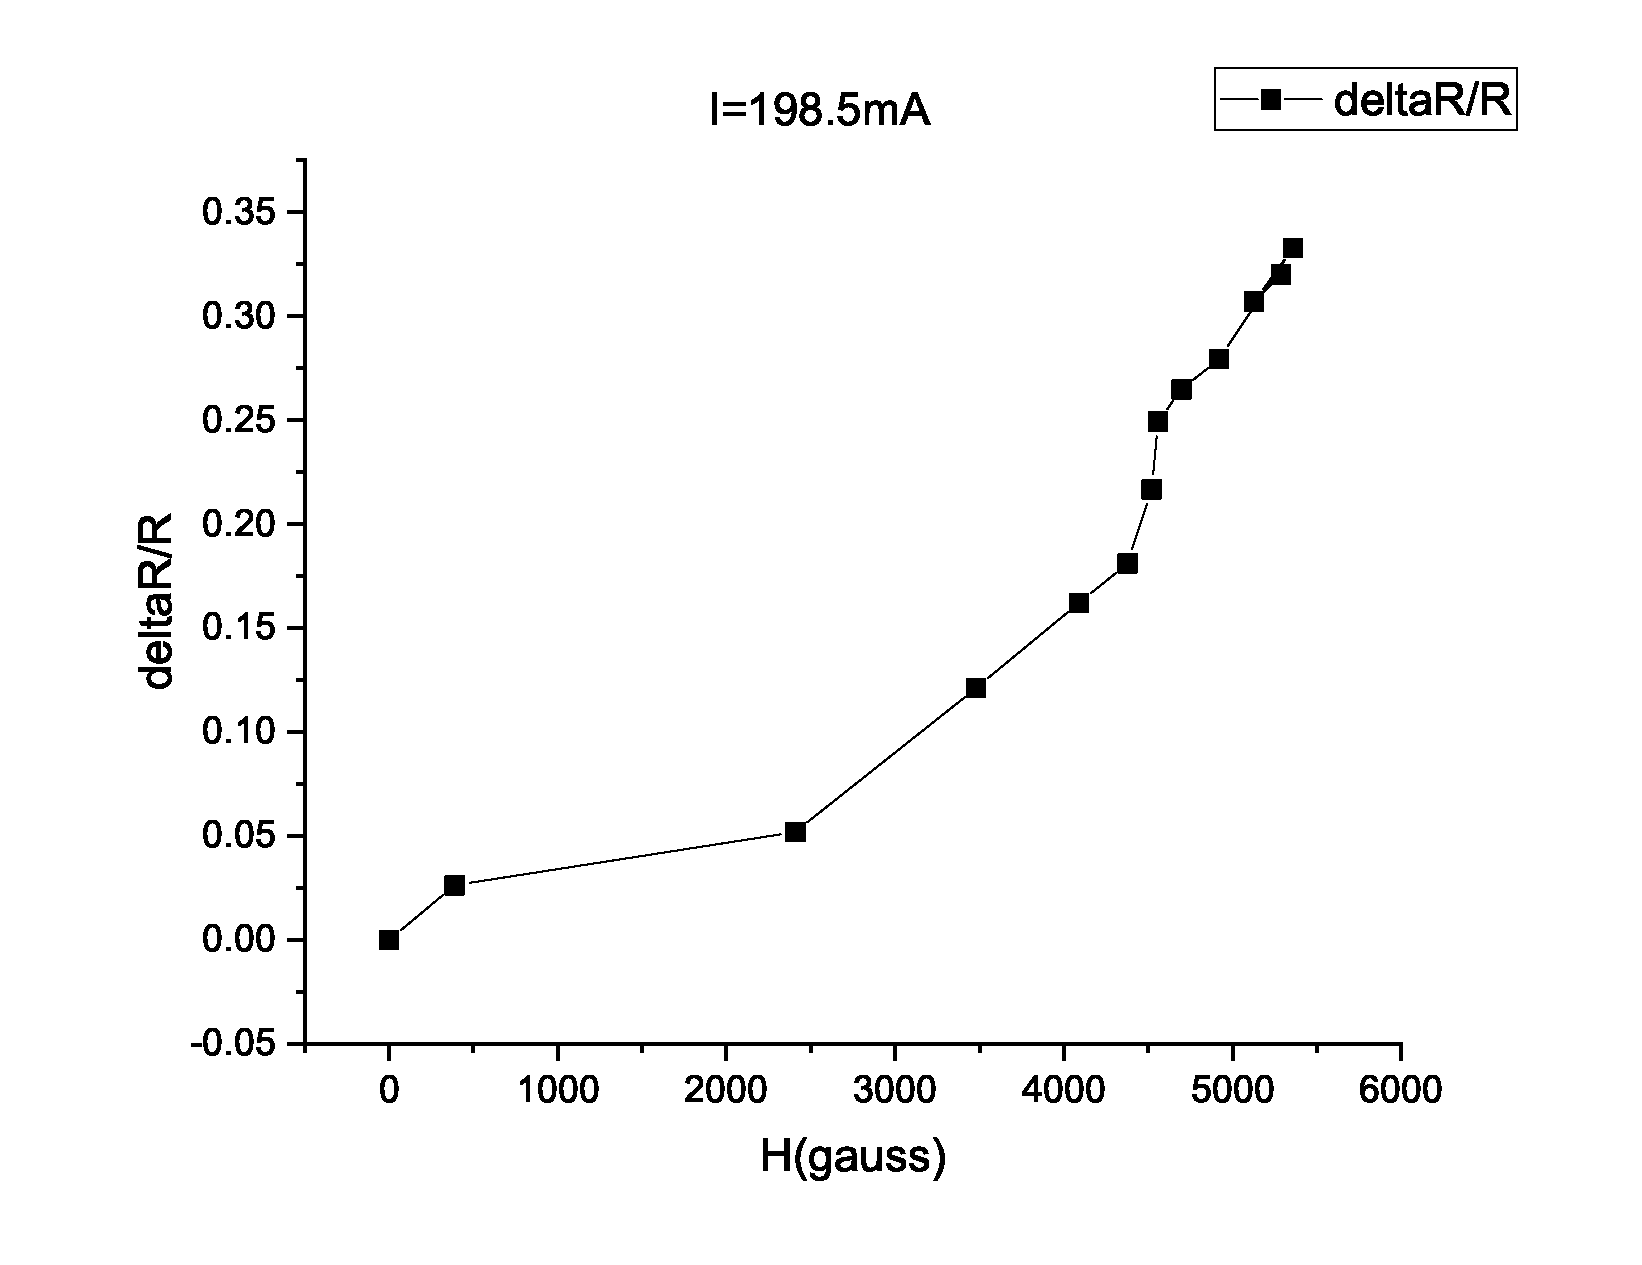
\includegraphics[width=90mm]{images/Graph1.eps}% Here is how to import EPS art
\caption{\label{fig:epsart} \((\Delta R)/R \)vs H}
\end{figure}
\begin{figure}[h!]
\centering
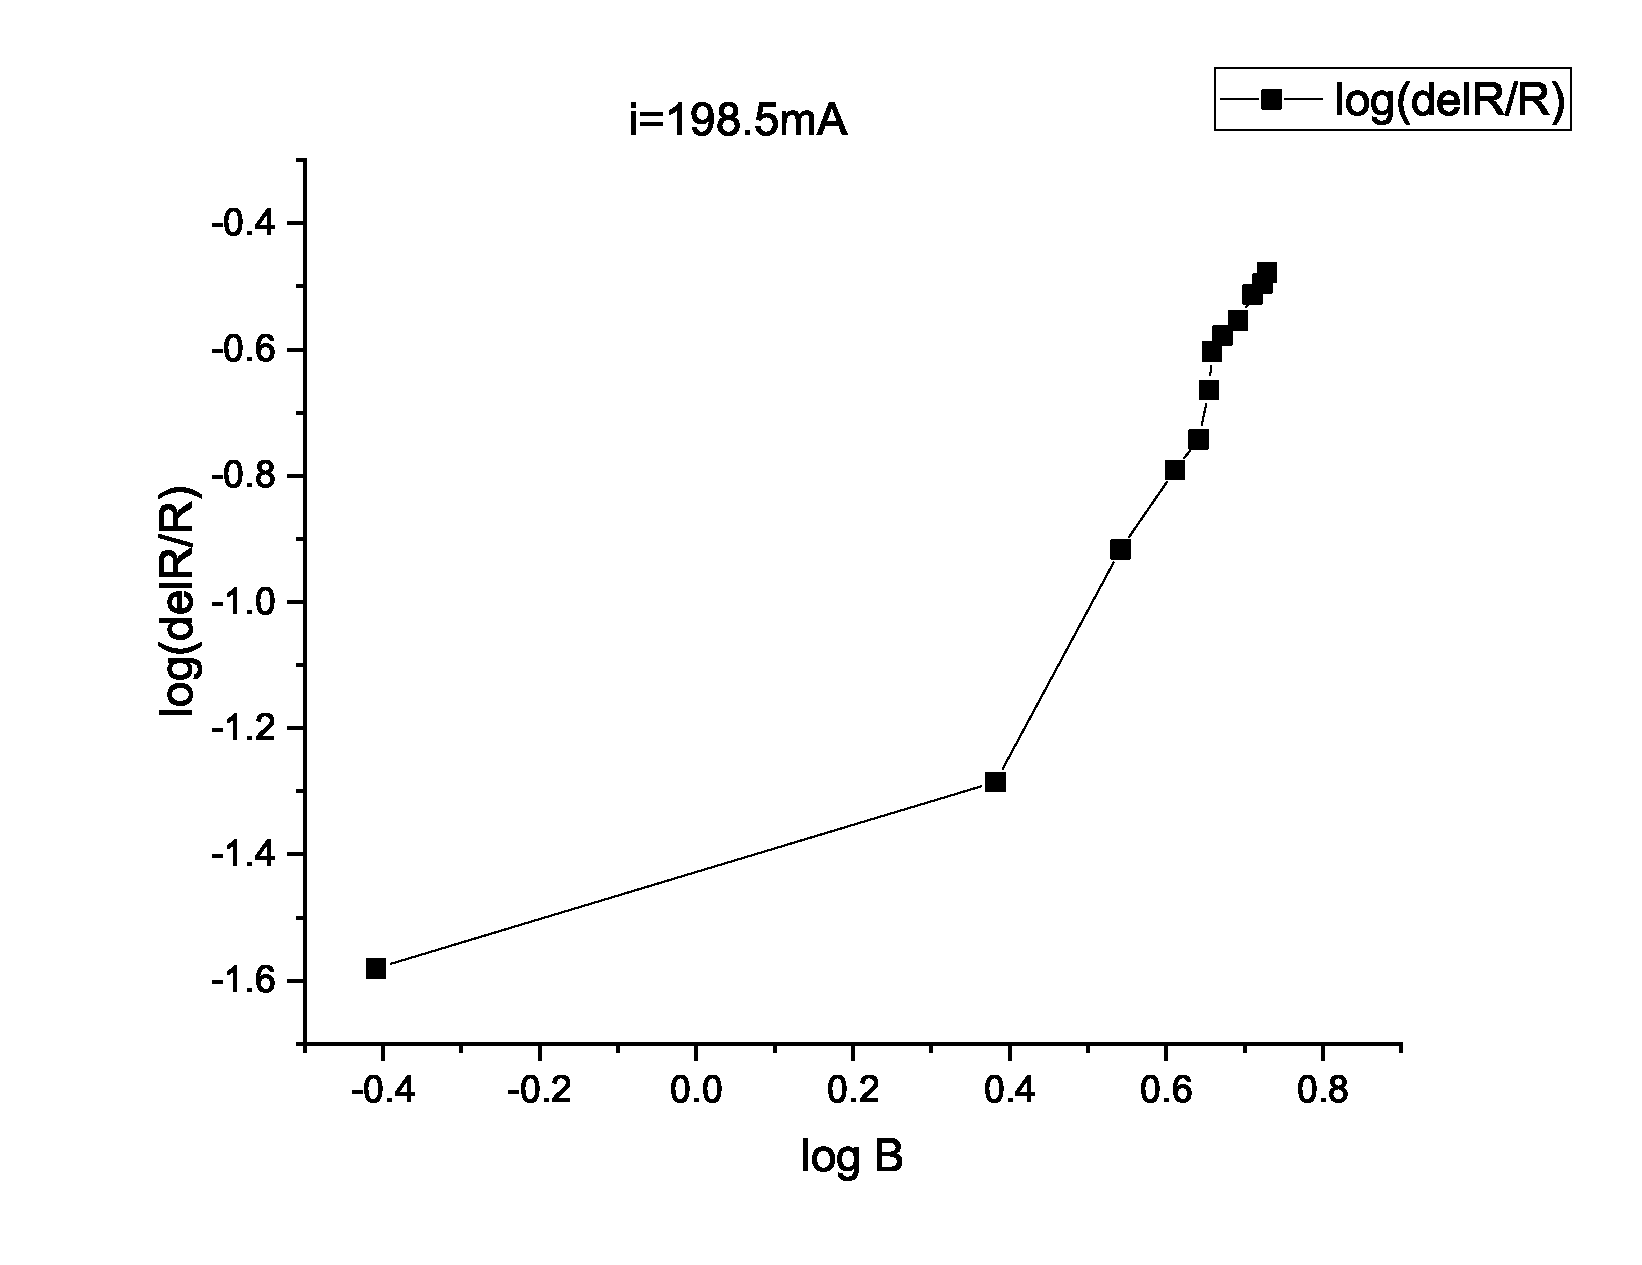
\includegraphics[width=90mm]{images/Graph2.eps}% Here is how to import EPS art
\caption{\label{fig:epsart} \(log (\Delta R/R)\)  vs log(H)}
\end{figure}


\subsubsection{I=101.0mA}
Table.2
\begin{table}[!ht]
    \centering
    \begin{tabular}{|l|l|l|l|}
    \hline
        H(gauss) & Voltage(mv) & Resistance & deltaR/R \\ \hline
        0 & 0.036 & 0.000183861 & 0 \\ \hline
        3330 & 0.037 & 0.000188968 & 0.026291892 \\ \hline
        4260 & 0.038 & 0.000194076 & 0.051915789 \\ \hline
        4670 & 0.041 & 0.000209397 & 0.121287805 \\ \hline
        4950 & 0.043 & 0.000219612 & 0.16215814 \\ \hline
        5120 & 0.044 & 0.000224719 & 0.1812 \\ \hline
        5380 & 0.046 & 0.000234934 & 0.2168 \\ \hline
        5800 & 0.048 & 0.000245148 & 0.249433333 \\ \hline
    \end{tabular}
\end{table}

\begin{figure}[h!]
\centering
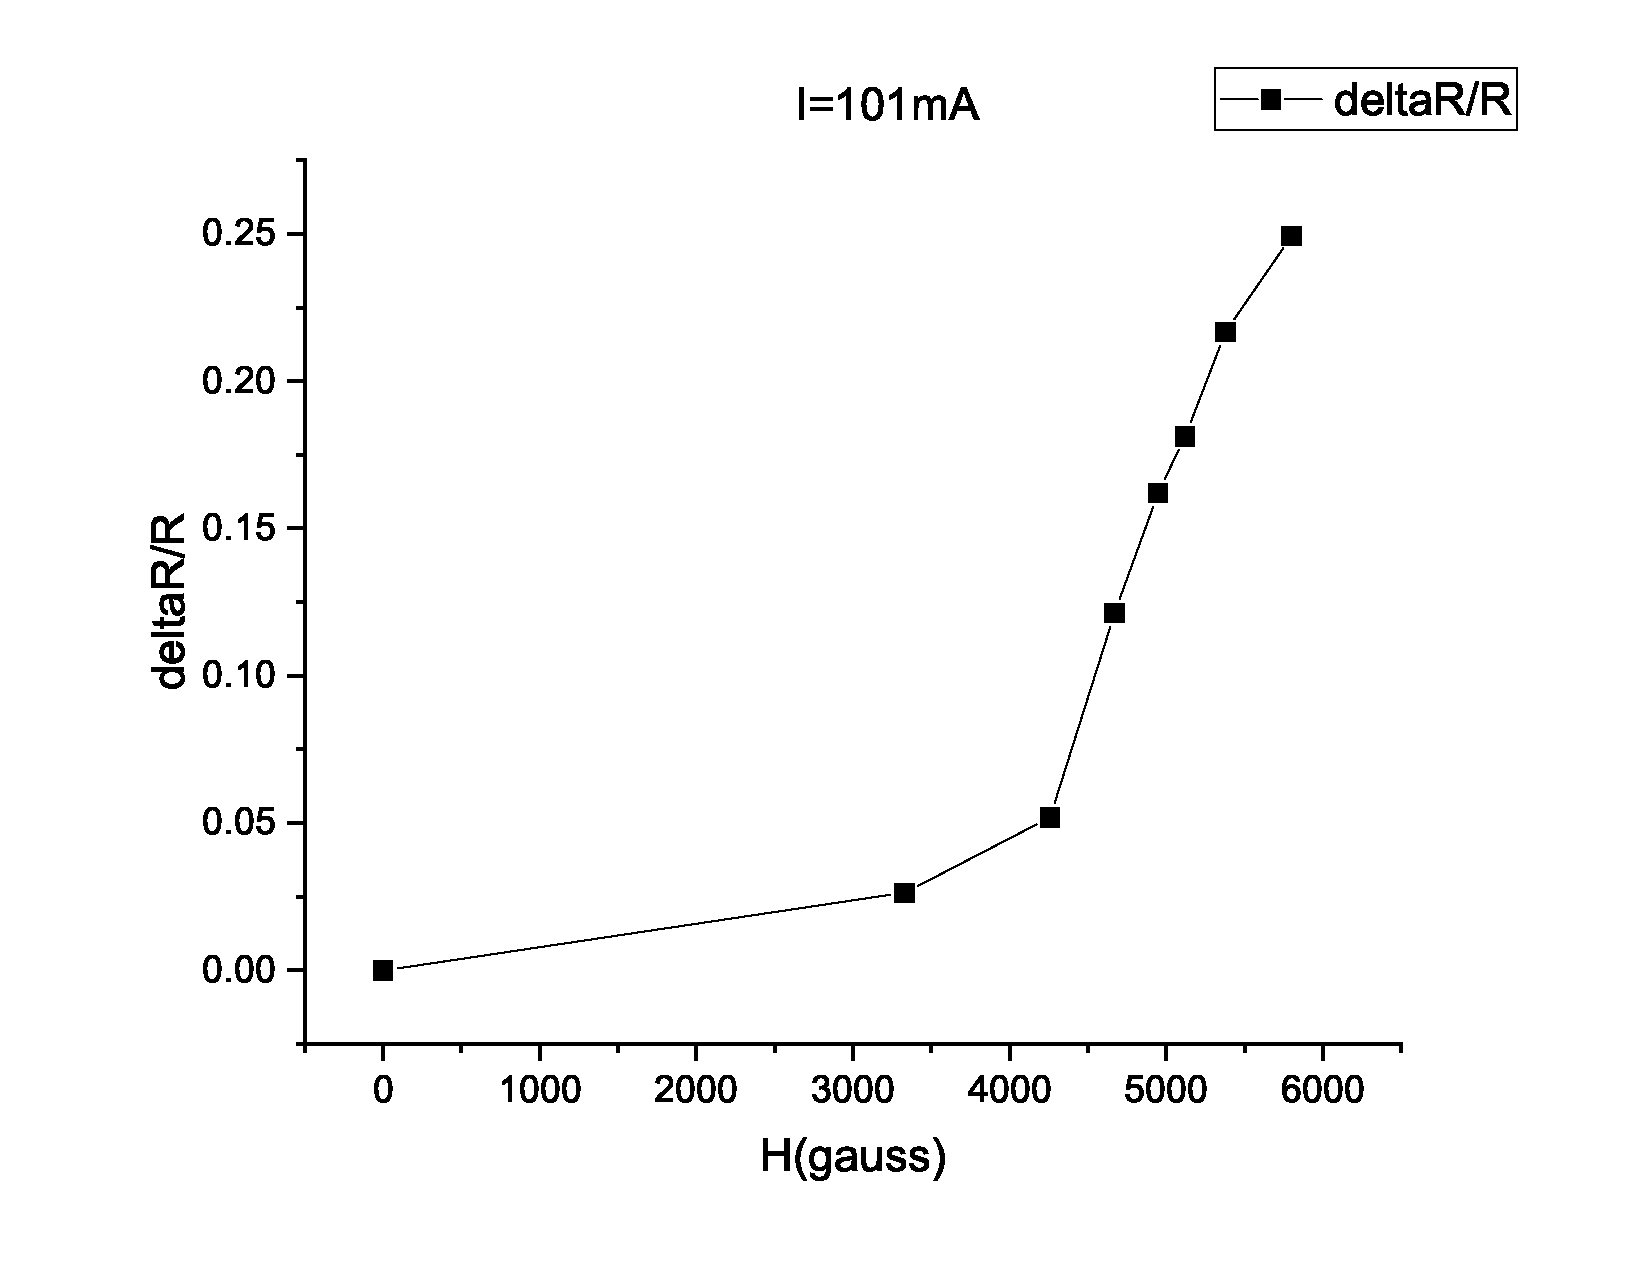
\includegraphics[width=90mm]{images/Graph3.eps}% Here is how to import EPS art
\caption{\label{fig:epsart} \((\Delta R)/R \)vs H}
\end{figure}
\begin{figure}[h!]
\centering
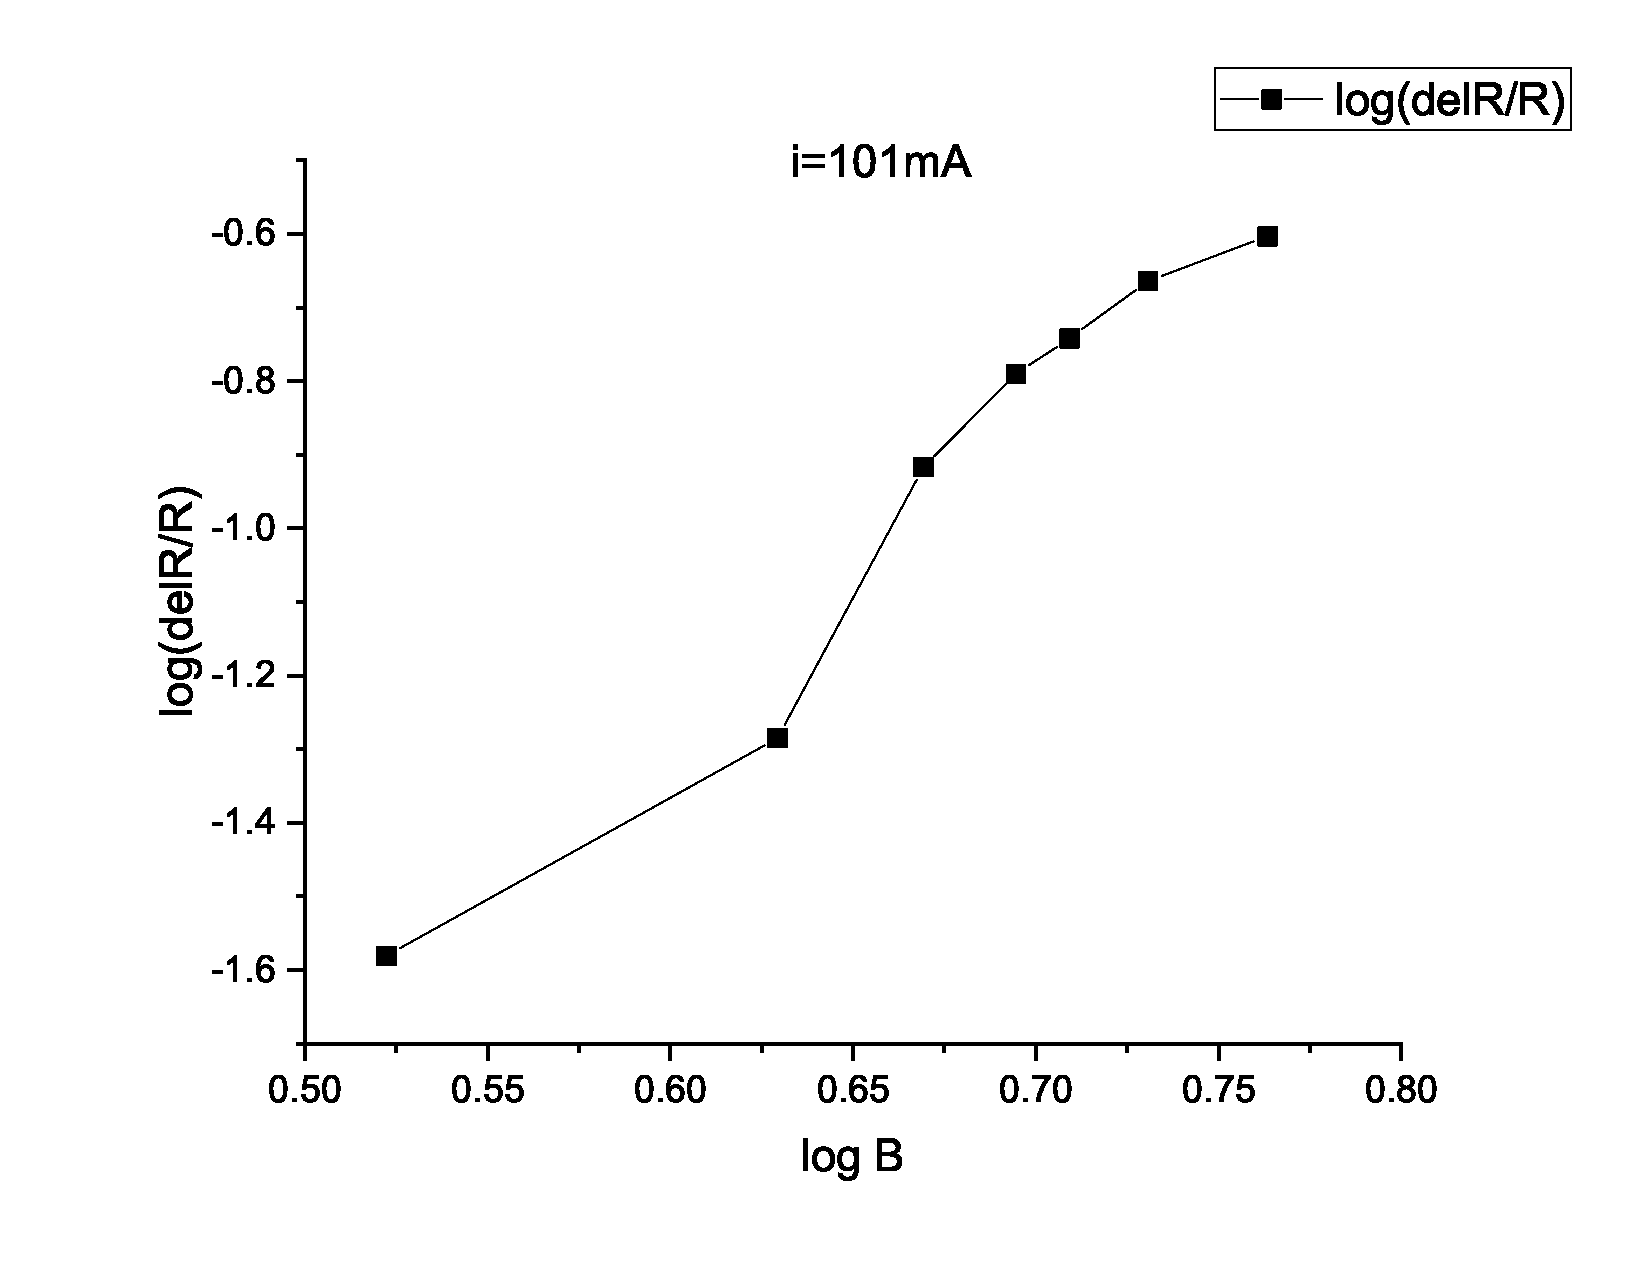
\includegraphics[width=90mm]{images/Graph4.eps}% Here is how to import EPS art
\caption{\label{fig:epsart} \(log(\Delta R/R)\) vs H}
\end{figure}

\subsection{Hall effect}
I=197.3mA\\
Room temperature=25$^{\circ}$ C\\
Thickness(z)=0.5mm\\
\\Table.3
\begin{table}[!ht]
    \centering
    \begin{tabular}{|l|l|}
    \hline
        H(gauss) & V(mV) \\ \hline
        2390 & -0.061 \\ \hline
        2540 & -0.062 \\ \hline
        3160 & -0.063 \\ \hline
        3480 & -0.064 \\ \hline
        4200 & -0.065 \\ \hline
        4500 & -0.066 \\ \hline
        4780 & -0.067 \\ \hline
        5200 & -0.068 \\ \hline
        5180 & -0.069 \\ \hline
    \end{tabular}
\end{table}
\begin{figure}[h!]
\centering
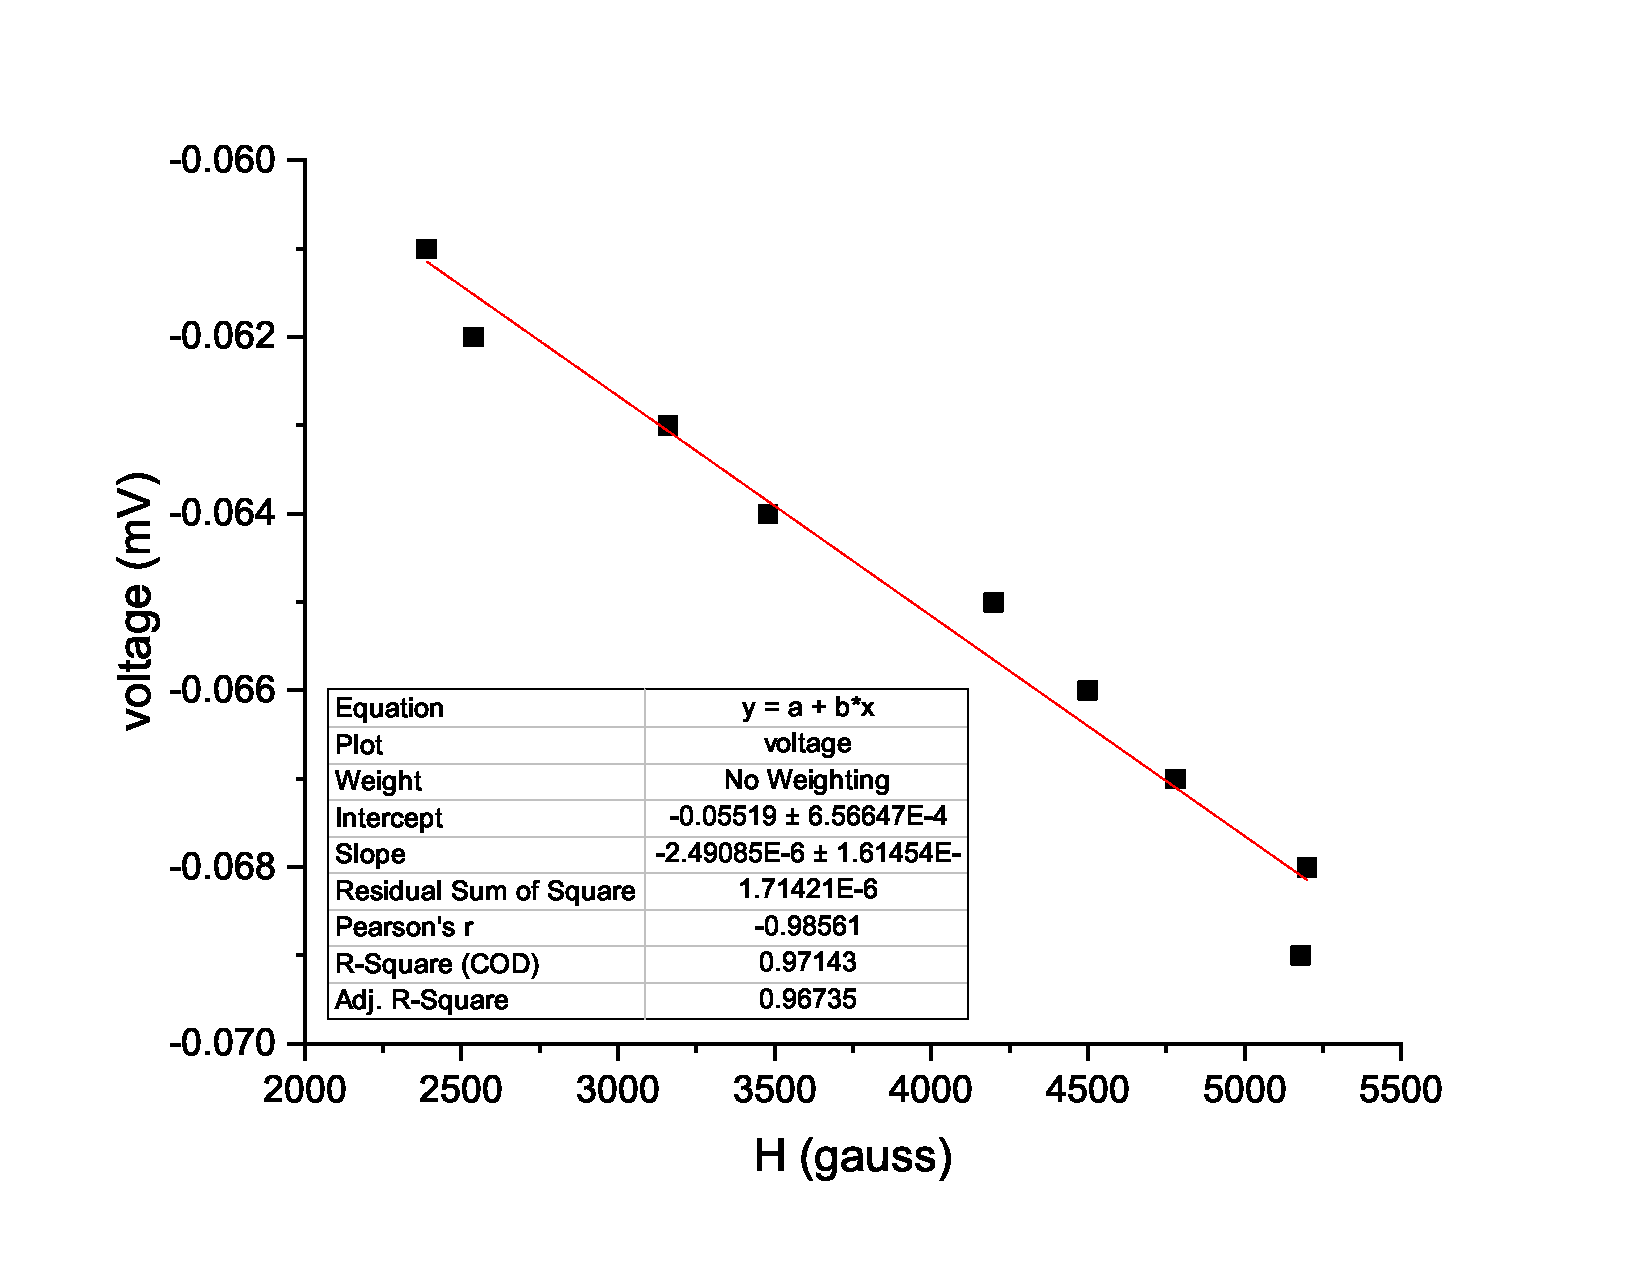
\includegraphics[width=90mm]{images/Graph6.eps}% Here is how to import EPS art
\caption{\label{fig:epsart} hall voltage vs H}
\end{figure}

from equation 2, we have\\
\(R=$$\frac{V_h z}{IH}$$\)\\
 \(R=$$\frac{slope *z}{I}$$\) ,\\hall coefficient, 
R=-6.951 x 10^-^1^2 ohm-cm /Gauss
 
\subsubsection{Error analysis}
we have, from equation 2, \\
\(($$\frac{\Delta R}{R}$$)^2=($$\frac{\Delta slope}{slope}$$)^2 + ($$\frac{\Delta I }{I}$$)^2\)\\
as z is error is not mentioned.
thus\\
\(\Delta R\)=+-0.45 x 10^-^1^2 ohm-cm/Gauss
\subsection{Data analysis}
We see that the magneto-resistance value increases with an increase in a magnetic field. The change is slow at low magnetic field intensity but increases as intensity increases. The reason could be due to an increase in Lorentz force on charge particles. we see that the change in resistance for Bismuth is 35 percent(i=198.5mA) and 25 percent(i=101mA) at the high magnetic field. The change in magneto-resistance decreases as the current operating decreases as the number of charge carrier decreases. Further, we can see that the curve deviates from the expected curve shape at the low operating current and  saturates at high temperatures due to limited charge carriers.\\
In the Hall coefficient, we see that the error in the Hall coefficient value is about 6 percent. The following deviation in data points could be due to increased temperature, as equipment heats up due to continuous use and fluctuation of room temperature. Another factor can be due to the residual magnetic field in coils at zero current(3 Gauss) and fluctuation of operating current. As we have \(R_h=1/ne \) thus charge density is high as expected in metals.